\chapter{Разработка алгоритма для игры NetHack с применением машинного обучения с подкреплением}\label{ch:ch3}

\section{NetHack - одна из самых сложных игр для RL}

Игра NetHack одна из старейших и наиболее популярных rouge-подобных игр. Первая версия игры появилась в 1987 году, а последняя вышла в 2020. В начале игры, герой оказывается в подземелье в котором он должен найти амулет Вендора. Для этого герой должен пройти более чем 50 процедурно генерируемых уровней. Игра имеет текстовый интерфейс представленный на рис.~\ref{fig:nethack_map}. В центре с помощью ascii символов изображается подземелье, сверху появляется текстовое сообщение описывающее положение в игре, а снизу содержится информация о состоянии героя. 

\begin{figure}[ht]
\centerfloat{
        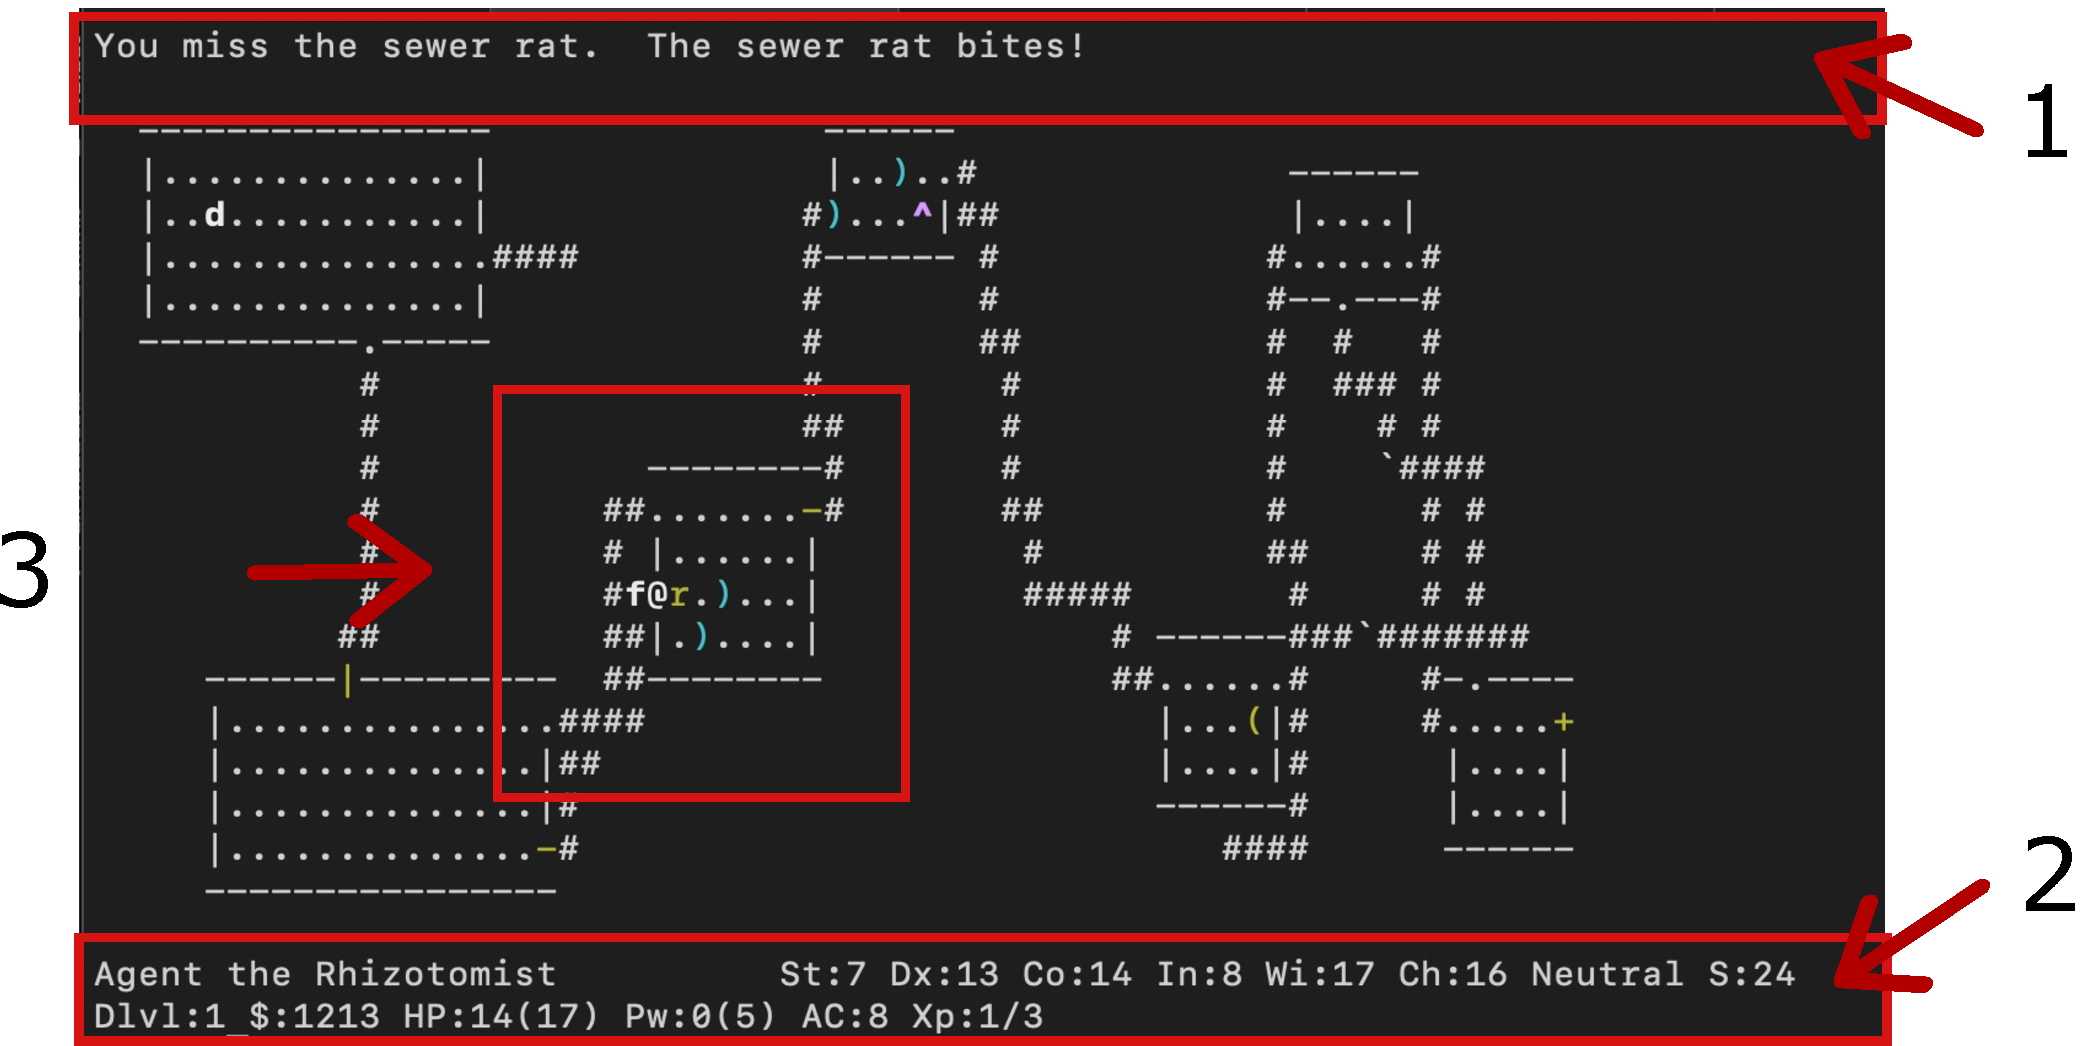
\includegraphics[width=0.85\textwidth]{images/nethack_map_view.pdf}
}
\caption{Интерфейс игры NetHack. (1) текстовое сообщение описывающее текущее событие, (2) статистика агента (здоровье, золото, сила, и др.) (3) окно центрированное возле текущего положения агента (@).}
    \label{fig:nethack_map}
\end{figure}

Несмотря на простой интерфейс NetHack ставит перед игроком сложные задачи. Далее опишем основные сложности которые делают NetHack серьезным испытанием как для человека, так и для RL агента.

\begin{itemize}
    \item \textbf{Процедурная генерация среды.} Многие компоненты игры являются процедурно генерируемыми и имеют случайную динамику. Например, точное положение интересующих объектов таких как расположение предметов, монстров, еды и также структура подземелий генерируются случайным образом. Использование процедурной генерации уровней приводит к тому, что агент практически никогда не попадет в точно такую же ситуацию в которой он был в прошлом. При обучении RL агентов это приводит к фундаментальной проблеме с количеством данных необходимых для обучения и позволяет оценить способность агента обобщать свою текущую стратегию на новые задачи. Также в игре NetHack не работают методы исследования среды Go-Explore \cite{ecoffet2019, ecoffet2021} основанные на стратегии, умеющей возвращаться в ранее посещенные состояния которые в других задачах показывают наилучшие результаты. Кроме того, состояние в игре NetHack состоит из сотен возможных символов, что приводит к огромному количеству возможных состояний. Более того, в игре NetHack у героя могут быть различные роли (например, монах, валькирия, волшебник, турист), расы (человек, эльф, гном, орк) и различные начальный набор предметов. 
    \item \textbf{NetHack -- очень длинная игра.} Эксперту для прохождения игры NetHack требуются десятки тысяч ходов. У среднего игрока прохождение игры может занять многие дни и более сотни тысяч ходов. По сравнению с другими тестовыми задачами для RL агентов такими как  StarCraft и Dota 2, эпизоды в NetHack на один или два порядка длиннее и сильно зависят от текущей стратегии агента. 
    \item \textbf{Много модальные наблюдения.} Как показано на рис.~\ref{fig:nethack_map} в текущее состояние агента входит графическое изображение карты и его положение на ней; сообщение на естественном языке описывающее текущее событие; числовые признаки описывающие состояние агента; категориальные признаки описывающие имеющиеся в распоряжении у агента предметы и особенные свойства агента. 
\end{itemize}

Также сложность игры подчеркивает то, что для NetHack существует обширное описание \cite{nethack_wiki} возможных стратегий поведения созданное активными игроками которое может быть использовано для обучения RL агентов. Кроме того, существует репозиторий с большим количеством записей реальных игроков \cite{alt} который может быть использован для обучения агента имитировать их стратегии. Таким образом NetHack ставит уникальные задачи для исследований в области применения RL агентов. 

\subsection{NLE - среда основанная на игре NetHack}
В работе \cite{nethack} авторами для игры NetHack была разработана среда NLE для обучения RL агентов на основе версии NetHack 3.6.6. Среда NLE удовлетворяет gym интерфейсу \cite{brockman2016openai} и позволяет обучать RL агентов в игре NetHack. Важной особенностью NLE является то, что она практически не ограничивает возможностей агента в игре и он способен совершать такие же действия, как и человек использующий стандартный интерфйес. 

\paragraph{Пространство состояний.}
By default, the observation space consists of the elements glyphs, chars, colors, specials, blstats,
message, inv\_glyphs, inv\_strs, inv\_letters, as well as inv\_oclasses. The elements glyphs, chars, colors,
and specials are tensors representing the (batched) 2D symbolic observation of the dungeon; blstats
is a vector of agent coordinates and other character attributes (“bottom-line stats”, e.g., health points,
strength, dexterity, hunger level; normally displayed in the bottom area of the GUI), message is a
tensor representing the current message shown to the player (normally displayed in the top area of
the GUI), and the inv\_* elements are padded tensors representing the hero’s inventory items. More
details about the default observation space and possible extensions can be found in Appendix B.

\paragraph{Пространство действий.} The environment has 93 available actions, corresponding to all the actions a human player can take in
NetHack. More precisely, the action space is composed of 77 command actions and 16 movement
actions. The movement actions are split into eight “one-step” compass directions (i.e., the agent
moves a single step in a given direction) and eight “move far” compass directions (i.e., the agent
moves in the specified direction until it runs into some entity). The 77 command actions include
eating, opening, kicking, reading, praying as well as many others. We refer the reader to Appendix C
as well as to the NetHack Guidebook [59] for the full table of actions and NetHack commands.

\paragraph{Награда.}

\paragraph{Эпизод.}


\section{Декомпозиция игры NetHack на подзадачи}

//TODO describe subtasks we choose. 

\begin{figure}[ht]
\centerfloat{
        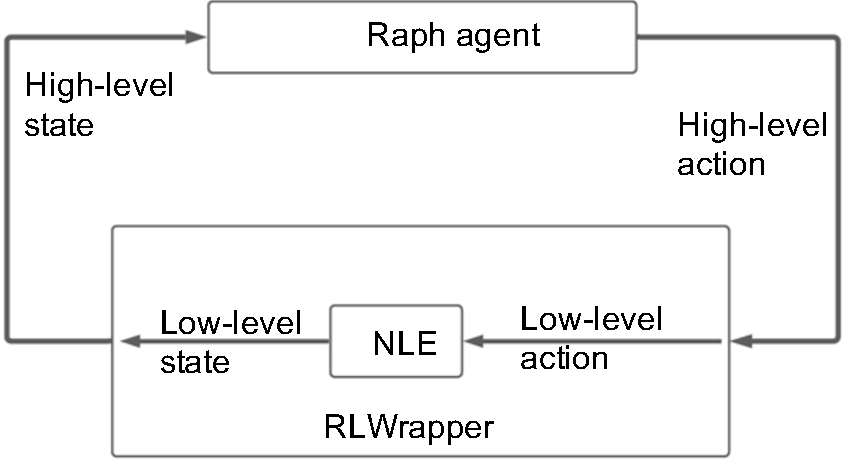
\includegraphics[width=0.75\textwidth]{images/raph_wrapper.pdf}
}
\caption{Схема взаимодействия RAPH агента со средой NLE.}
    \label{fig:raph_nle}
\end{figure}


\section{Обучение иерархического агента совмещающего обучение с подкреплением и алгоритмический подход}


We decided to apply a hierarchical approach to the challenge and construct an agent's policy from basic skills dedicated to solving concrete tasks: eating, fighting, dungeon exploration, and inventory management. The approach closely resembles the options framework of \cite{Sutton1999}, in which a higher-level policy orchestrates the execution of eligible lower-level options until termination. This modularity allows us to build a hybrid neural-algorithmic method, where some skills can be trained, and others -- hard-coded.
%
In our case, we opted for a simplified higher-level policy and implemented it as a rule-based algorithmic decision system, that executes a lower-level skill on a first-fit basis. The priority and triggers of each skill were designed manually and determined based on our expert knowledge of rogue-likes and essential game AI.

One of the most important and complex skills, which accounts for the bulk of in-game score, is battling monsters. Fighting and combat require a complex policy to assess the surrounding topology of the level and choose an appropriate action: approach, outflank, avoid getting surrounded, decide on a melee or ranged attack, heal, wait or flee.
%
To this end we train a deep neural RL agent based on the TorchBeast baseline, provided in \cite{kuettler2020nethack}, to learn a policy for the lower-level fighting skill. The agent has a discrete action space containing \emph{eight} actions for directional movement or melee attacks, another \emph{eight} actions for directional ranged attacks, and \emph{three} actions for hard-coded composite controls such as waiting, praying and engraving ``Elbereth'', the latter warding off low-level aggressive monsters.
%
The neural policy uses hand-crafted features related to the map, monster, and hero's vitals, extracted by the lower level algorithmic dungeon level mapping subsystem of the agent.
%
We implement other skills as hard-coded algorithmic policies based on graph navigation algorithms and expert knowledge.

To train the agent we construct episodes by \emph{pasting contiguous fragments} with transitions in which there is a \emph{hostile monster within the field-of-view} of the agent. In other words, the steps performed by all other skills are ``fast-forwarded'', which makes the environment a partially observed semi-Markov decision process from the point of view of the agent, \cite{Sutton1999}.
%
The inference of our RAPH agent works as presented in the Appendix, in algorithm~\ref{alg:raph}. If necessary, we first handle pending NetHack's GUI events, such as responding to multi-part message logs. Next, we parse and update the dungeon representation and extract the features for the neural agent. Finally, we sample actions from either the RL agent or the hard-coded skill, whichever one currently holds control, taking into account the distance to the nearest monster.


Analysis of a trained policy shows that move or melee attack actions are used in 66\% of steps, range attack in 21.6\%, wait in 11\%, ``Elbereth'' in 0.3\%, and pray in 0.1\%. 




\begin{algorithm}[H]
\SetKwComment{Comment}{/* }{ */}
\SetKw{Continue}{continue}
\caption{RAPH agent}\label{alg:raph}
\KwData{view\_distance, agent, hard\_coded\_skills}
$state, done \gets env.reset(), False$\;

\While{not done}{
  action\_queue = parse\_message(state)\;

  \If{action\_queue} {
   state, reward, done, info = env.step(action\_queue)\Comment*[r]{We have a prompt to response}
   \Continue
  }

  monster\_distance, preprocessed\_state = parse\_dungeon(state)\;
  \eIf{monster\_distance \textless view\_distance}{
    action\_queue = agent.act(preprocessed\_state)\;
  }{
    action\_queue = first\_fit(hard\_coded\_skills, preprocessed\_state)\Comment*[r]{Select non-rl action on first-fit basis}
  }
  state, reward, done, info = env.step(action\_queue)\;
}
\end{algorithm}


\begin{figure}[ht]
\centerfloat{
        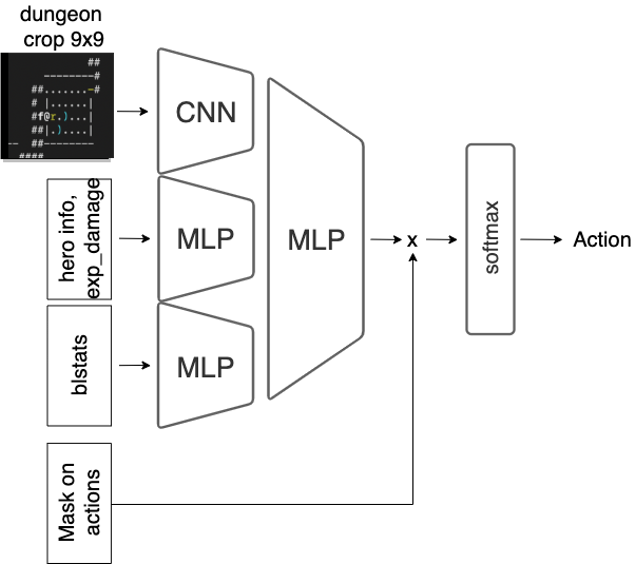
\includegraphics[width=0.5\textwidth]{images/raph_arch.png}
}
\caption{NN architecture}
    \label{fig:raph_arch}
\end{figure}

\begin{figure}[ht]
\centerfloat{
        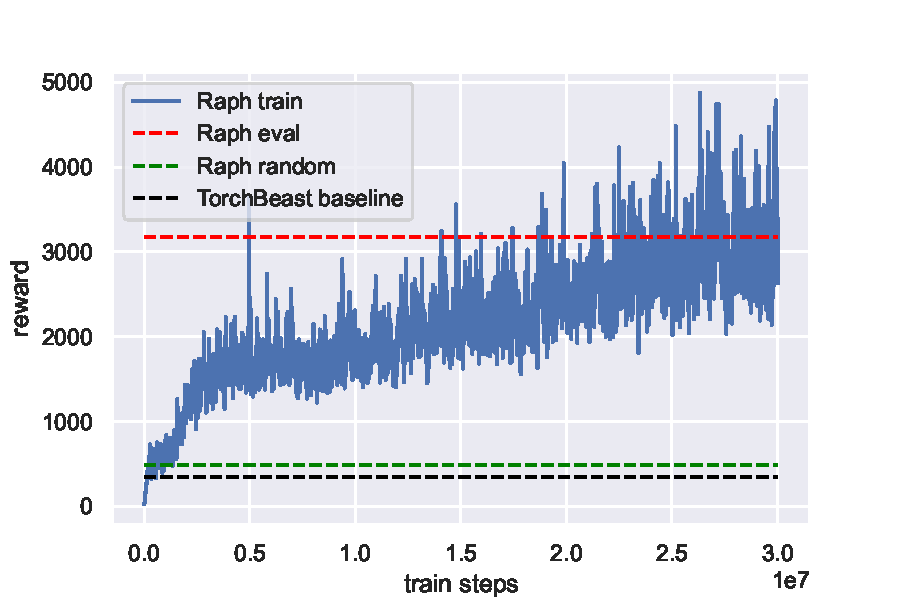
\includegraphics[width=0.95\textwidth]{images/raph_train.pdf}
}
\caption{Exponentially moving average of reward during training}
    \label{fig:raph_train}
\end{figure}

\section{Выводы}

\clearpage
